\chapter{General Architecture}
\label{chapter:architecture}

This section presents the main guidelines of the architecture used in developing the BLEOffloadingFramework and the two main offloading solutions. The first topic of discussion is the environment in which the framework is run, followed by the presentation of the techniques used and finally a general description of the data flow.

\subsection{Offload Environment}
\label{environment}

When talking about offloading in a mobile context, we mainly refer to transferring code and data from hand held devices. These devices have evolved in recent years from the mobile phones used to communicate between two or more people to personal computers that permit you to connect to the Internet, socialize, play videos, listen to songs and much more. On the current market, the lead operating systems for smart phones are Android, open source project maintained and controlled by Google, and iOS, proprietary software owned by Apple.

Because of its open source nature and the fact that it is present on different devices with different specifications, the BLEOffloadingFramework was built with Android as the primary client for this architecture. Although, the generic approach devised here accounts for any smart phone that has the capability of Bluetooth Low Energy technology.

Android is an operating system based on the Linux kernel \footnote{www.kernel.org} with enhancements regarding embedded systems, such as a well defined sleep/idle time, better power management, paranoid security and a well rounded framework that acts as a layer between underlying hardware and software applications. The Android Framework is mainly written in Java and has a client-server approach to inter process communications and event managing.

This approach permits applications developed by third parties to be created and run inside their own virtual machine and whenever they need a system functionality, such as access to the camera hardware or to other applications a request needs to be sent through the framework. An overview of Android and its functionality can be viewed at \cite{Android}.

As such, the environment that the offloading framework proposed in this paper is defined as the Android mobile applications and one of the main objectives of the project is to help developers in creating power saving applications using this system.

\subsection{Offloading Solutions}
\label{offloadingsolutions}

After defining the objective and the clients of this framework, it is time to define the general offloading methods through which the system achieves its purpose.

\begin{enumerate}

\item{\emph{Remote Procedure Call/Remote Method Invocation}}

RPC\cite{RPC} is not a new protocol. With the advent of the Internet, which has become the largest distributed system ever built, several methods of accessing code across different platforms have been described for different uses: from database interrogation across networks to accessing the output of proprietary code in a secure way. The basic definition of RPC is that it's similar to local procedure call in the way that when a section of code desires to call a procedure it would need an address to jump to. In Remote Procedure Call, that address can be on another machine altogether and the system can either wait for the procedure to finish, or, in more complex systems, continue it's execution and receive an event when the call is done. 

For offloading purposes, RPC or RMI (the equivalent in object oriented languages) means that the device can effectively use a system that has been implemented and stabilized for some time now in order to execute very processor intensive code. This would be the main advantage regarding this offload technique.

The main disadvantage would be that it is not a very scalable solution. A developer that uses Remote Procedure Calls would have to plan its application in advance and select the exact methods or procedure that he wishes to offload. This sometimes results in duplicate code, as the framework would not be available some times, and would be very hard to maintain.

\item{\emph{Loose coupling of systems}}

If the previous method relies solely on implementation, this method requires structuring the application in such a way that certain parts are independent from the rest of the system, as shown in figure \ref{looseimage}.

A good example is an application that processes images in order to obtain certain information from it, such as faces or objects. If we are to take into consideration hand held devices without a specialized Graphical Processing Unit, then this algorithm is costly on the CPU. In these cases, it would be much more efficient to send the picture to another device and use its processing power or even GPU.

The drawback of this method is that not all applications are suited for this type of design (such an application that rely solely on device hardware), while the advantage is that it offers a scalable approach to offloading.

\end{enumerate}

%\begingroup
%	\centering
%	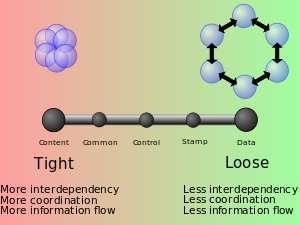
\includegraphics[scale=0.5]{CoupledLoose.png}
%	\captionof{figure}{Tight and Loose Coupled systems\cite{wikitight}}\label{looseimage}
%\endgroup

\subsection{Data flow and main agents}
\label{dataflow}

In a general Offloading Framework three components can be correctly identified: the device that needs to offload its work, the communication channel and the the device that helps boost performance and receives the work to be offloaded.
%\TODO Name the ofloadee and the ofloaded

The system proposed in this paper uses for communication a low power consumption implementation of the Bluetooth technology, called Bluetooth Low Energy \cite{BLE2}. This technology permits a high throughput of data to be transferred wireless with relatively low energy consumption over short distances ( below 10 meters ). The benefit the BLE communication brings is that the channel used has a very low impact on the system itself \cite{BLE}, but it has an innate drawback in the fact that it has a short range.

In order to mitigate this drawback, in this framework the device that provides the processing power is a small System on a Chip device that can either lend its power to mobile devices or act a gateway to other more powerful systems. The benefits for adding an intermediary for offloading solutions is that it keeps the simple goal of preserving battery power on the mobile device. The SoC is a small computer, without a battery that can be positioned almost anywhere: in a home, public transportation stations or work environments. By offering the possibility to access different processing power nodes would significantly reduce the mobile devices battery consumption.

Moreover, the implementation of the system permits interchangeability between the client and server devices. As such, if a device permits it, it can act as a server for another device, and thus managing to share some of the resources. The model proposed here will assume that the client is a mobile device based on the Android OS, while the server is a SoC, specifically a RaspberryPI (An ARM GNU/Linux box for \$25).

In a first stage, when a piece of code that can be offloaded is detected, the client device will scan for potential offloading nodes. If such a node is detected, it will try to connect and create a network between the two devices. Once the connection is established, the client will send it's offloading request, through either of the aforementioned methods. The server will respond with either request acknowledge or busy.

The server can accept a number of connections and requests per time frame, in order to not burden itself and thus becoming a bottle neck for the system as a whole. Once the request has been acknowledged and processed, the results will be sent back to the mobile device, depending on the offload method that is used. An exemplification of this data flow can be view in figure \ref{btoffload}.
